% https://www.ual.es/estudios/masteres/presentacion/plandeestudios/trabajofinestudios/7114
% https://www.ual.es/application/files/6715/8764/9174/Plantilla_AnteProyectoTFM.docx

\documentclass[titlepage, 12pt, a4paper, oneside]{article}
\usepackage[utf8]{inputenc}
\usepackage[spanish, es-tabla]{babel}
\usepackage[T1]{fontenc}
\usepackage{hyperref}
\usepackage[numbib]{tocbibind}
\usepackage{tikz}
\usepackage[top=1in, bottom=1.25in, left=1.25in, right=1.25in]{geometry}
\usepackage{xcolor}
\usepackage{eso-pic}

\usepackage{fancyhdr}
\pagestyle{fancy}
\fancyhf{}
\rhead{\textit{\color[rgb]{0.0,0.424,0.616}Nombre del estudiante}}
\lhead{}
\rfoot{}
\renewcommand{\headrulewidth}{0pt}

\usepackage{pgfgantt}

\title{}
\date{}
\renewcommand{\familydefault}{\sfdefault}

\begin{document}
\thispagestyle{empty}
\tikz[remember picture,overlay] \node[opacity=1.0, inner sep=0pt] at (current page.center){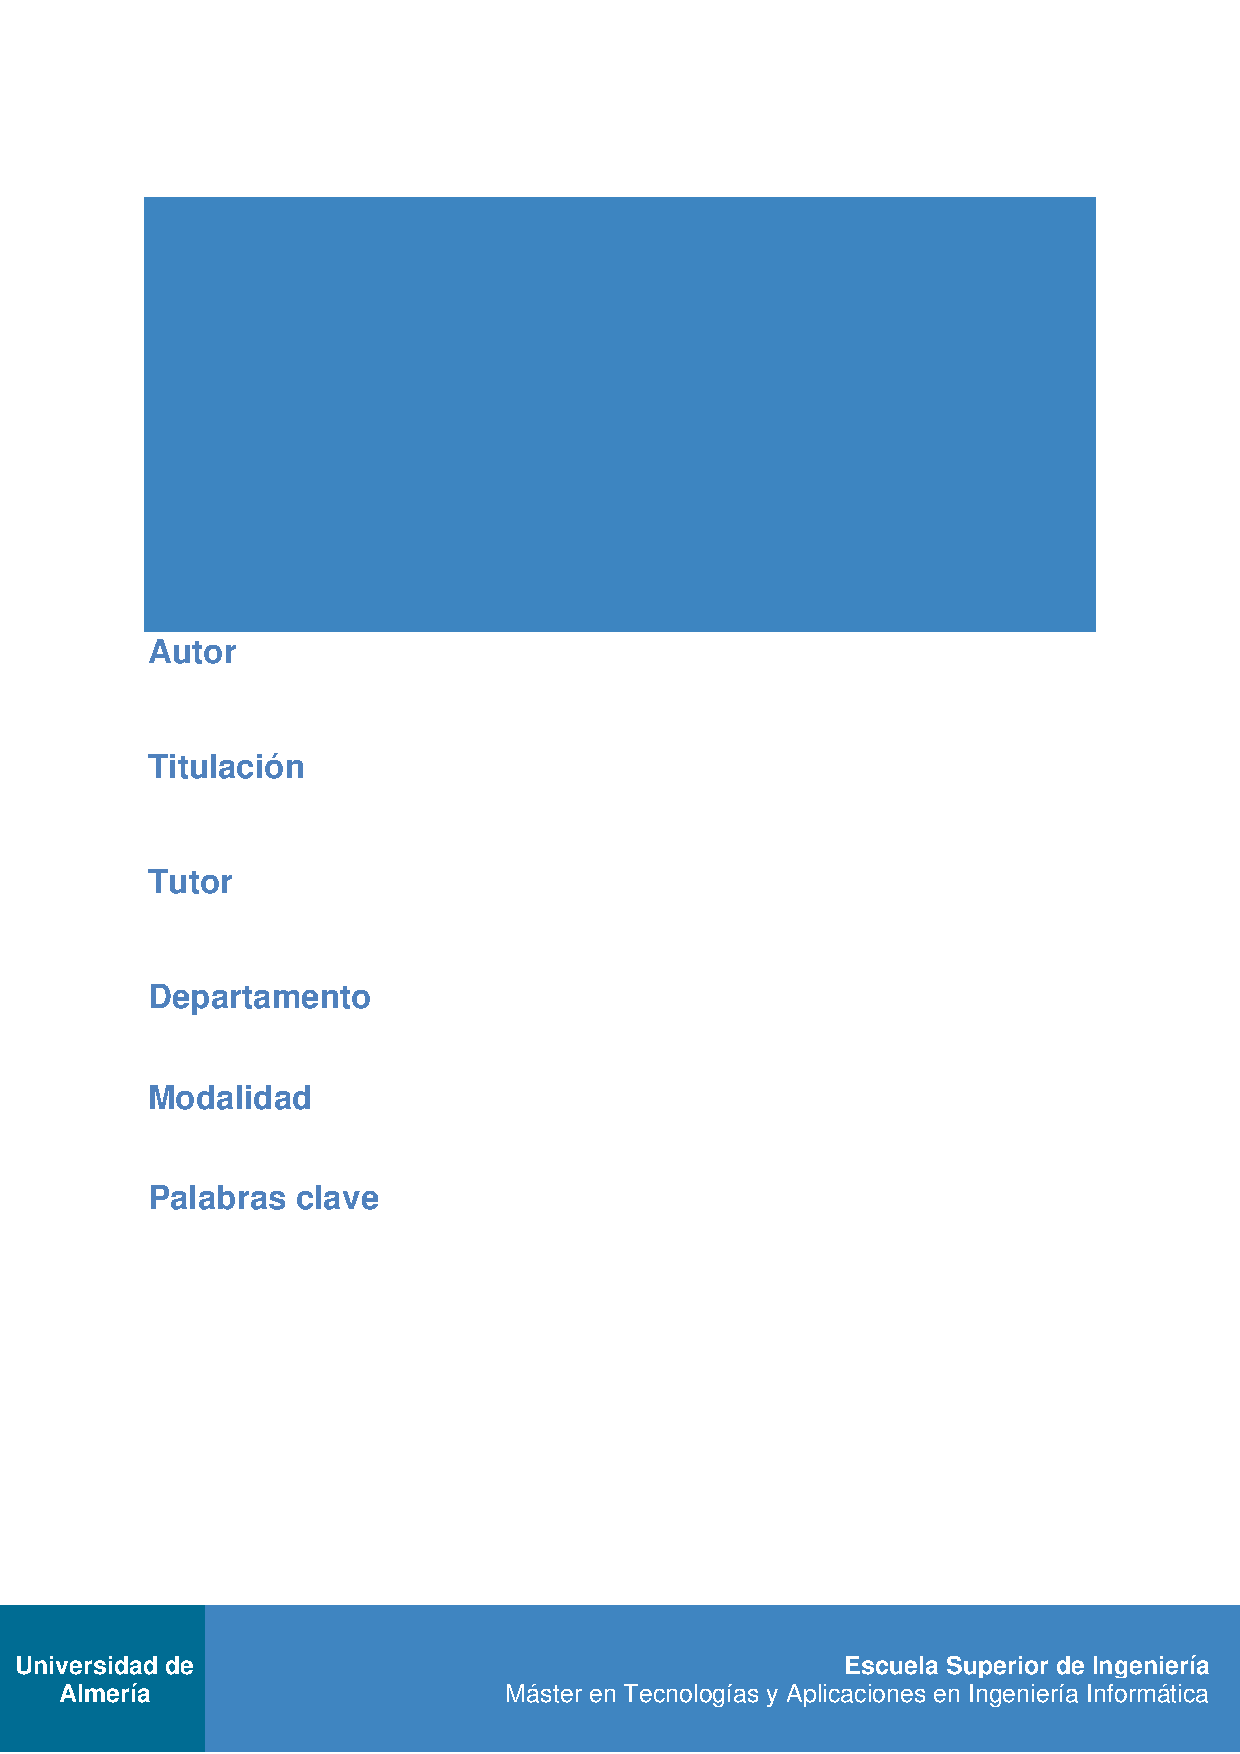
\includegraphics[width=\paperwidth,height=\paperheight]{Plantilla_AnteProyectoTFM-portada}};

\begin{center}
  \vspace{6cm}
  {\color{white} \Huge \textbf{Título del Proyecto}}
\end{center}

\Large

\vspace{-0.2ex}
\begin{tabular}{ll}
  ~~~~~~~~~~~~~~~~~ & Nombre del estudiante
\end{tabular}

\vspace{1.1cm}
\begin{tabular}{ll}
  ~~~~~~~~~~~~~~~~~ & Máster en Tecnologías y Aplicaciones \\
  & en Ingeniería Informática
\end{tabular}

\vspace{0.4cm}
\begin{tabular}{ll}
  ~~~~~~~~~~~~~~~~~ & Vicente González Ruiz
\end{tabular}

\vspace{1.1cm}
\begin{tabular}{ll}
  ~~~~~~~~~~~~~~~~~ & Departamento de Informática
\end{tabular}

\vspace{0.95cm}
\begin{tabular}{ll}
  ~~~~~~~~~~~~~~~~~ & Trabajo Técnico o Trabajo de Investigación % Elimina no que no proceda
\end{tabular}

\vspace{0.95cm}
\begin{tabular}{ll}
  ~~~~~~~~~~~~~~~~~ & Bla, bla, bla
\end{tabular}

\clearpage

% https://tex.stackexchange.com/questions/527456/background-image-on-every-page-with-tikz
\AddToShipoutPictureBG{\tikz[remember picture, overlay] \node[opacity=1.0,inner sep=0pt] at (current page.center){
\includegraphics[width=\paperwidth,height=\paperheight]{Plantilla_AnteProyectoTFM-paginas}};}

\normalsize

\section{Introducción}
\cite{einstein1922kosmologische}
En esta sección se comentarán las características del problema a resolver, los antecedentes del TFM y la justificación del mismo.

\section{Objetivos}
En esta sección se comentará el objetivo principal a conseguir en este TFM y los sub-objetivos necesarios para llevarlos a cabo.

\section{Fases de desarrollo}
En esta sección se comentarán las distintas fases en las que se ha dividido el trabajo a realizar.

Se contemplan las siguientes unidades de trabajo (total: 300 horas, véase la Figura~\ref{fig:temporizacion}):
\begin{enumerate}
  \item {ESTUDIO:} Estudio de transformadas, transformadas discretas,
    codificación de sub-bandas y filtrado por paso de sub-bandas y
    flujo óptico de imagen (60 h).
  \item {IDENTIFICACIÓN}: Identificación y selección de bibliotecas disponibles para
    cálculo óptico de imagen en el estado de arte actual (40 h).
  \item {INSTALACIÓN}: Instalación y configuración de las bibliotecas en el entorno
    de desarrollo (30h).
  \item {DESARROLLO}: Desarrollo para el cálculo de la estimación del flujo óptico
    de imagen (50h).
  \item {IMPLEMENTACIÓN}: Implementación del cálculo de la estimación del flujo óptimo
    al códec MCDWT (50h).
  \item {EVALUACIÓN}: Evaluación y pruebas del códec MCDWT (20h).
  \item {IMPLANTACIÓN}: Identificar limitaciones o incompatibilidades de hardware y
    software en otros dispositivos/plataformas de las bibliotecas
    usadas (20h).
  \item {REDACCIÓN}: Redacción y correcciones de la memoria previas a la
    presentación del TFM (30h).
\end{enumerate}

% Y en esta figura describe el desarrollo temporal de las anteriores fases. Rercuerda que en total deben sumar 300 horas.
\begin{figure}
  \begin{center}
    \resizebox{\columnwidth}{!}{
      \begin{ganttchart}{1}{30}{10}
        \gantttitle{Bloques de 10 horas}{30} \\
        \gantttitlelist{1,...,30}{1} \\
        \ganttbar{REV. BIB.}{1}{5} \\ % 50h
        \ganttlinkedbar{REV. SOFT.}{6}{10} \\ % 50 h
        \ganttlinkedbar{CONF. \& PRUEBA}{11}{15} \\ % 50 h
        \ganttlinkedbar{BATERÍA}{16}{20} \\ % 50 h
        \ganttlinkedbar{EVALUACIÓN}{21}{25} \\ % 50 h
        \ganttlinkedbar{REDACCIÓN}{26}{30} % 50 h
      \end{ganttchart}
    }
  \end{center}
  \caption{Temporización del trabajo.\label{fig:temporizacion}}
\end{figure}

\section{Materiales y métodos}
En esta sección se comentarán los diferentes materiales o herramientas y métodos o técnicas necesarias para la realización del TFM.

\bibliographystyle{plain}
\bibliography{../bibliografia}

\vspace{5ex}

\begin{center}
  \textbf{Firmas de los tutores}
\end{center}

\end{document}
